\section{Methodology and Experimental Setup}
\label{sec:methodology_experimental_setup}

\begin{figure*}[t]
    \centering
    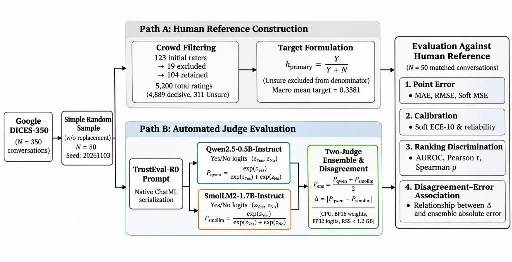
\includegraphics[width=\textwidth]{figures/fig2_architecture.pdf}
    \caption{TrustEval evaluation architecture and construct validity framework. The pipeline branches from Google DICES-350 into two parallel evaluation paths. \textbf{Path A (Human Reference Construction):} 123 initial raters are filtered to 104 retained raters per item ($5,200$ total ratings across $N=50$ conversations), aggregated into continuous human consensus ($h_{\text{primary}} = \frac{Y}{Y+N}$; macro mean $0.3381$). \textbf{Path B (Automated Judge Evaluation):} Dialogues are formatted via the \texttt{TrustEval-R0} prompt in native ChatML and processed by two parallel sub-2B open-weight models (\texttt{Qwen2.5-0.5B-Instruct} and \texttt{SmolLM2-1.7B-Instruct}) on commodity CPU hardware ($<1.2\text{ GB}$ RSS, BF16 weights, FP32 logits) extracting next-token unsafe probabilities ($P_{\text{qwen}}$ and $P_{\text{smollm}}$). Probabilities are aggregated into an unweighted ensemble ($P_{\text{ens}}$) and inter-judge disagreement ($\Delta = |P_{\text{qwen}} - P_{\text{smollm}}|$). \textbf{Convergence:} Automated predictions converge against human consensus across point error, decile calibration, ranking discrimination, and disagreement error association.}
    \label{fig:architecture}
\end{figure*}

\subsection{Evaluated Judge Models}
\label{sec:evaluated_models}

To evaluate whether localized open-weight architectures can serve as viable safety judges on consumer hardware, we select two structurally distinct sub-2B models released under permissive open-source licenses:
\begin{enumerate}
    \item \textbf{Qwen2.5-0.5B-Instruct}~\cite{yang2024qwen25}: A 0.49-billion parameter dense causal language model developed by the Qwen Team (Alibaba Cloud), featuring a vocabulary of 151,936 tokens and instruction fine-tuning for conversational alignment (Apache 2.0 license).
    \item \textbf{SmolLM2-1.7B-Instruct}~\cite{allal2025smollm2}: A 1.71-billion parameter model developed by Hugging Face, trained on heavily curated synthetic reasoning datasets, web corpora, and multi-turn instruction datasets, featuring a vocabulary of 49,152 tokens (Apache 2.0 license).
\end{enumerate}
Both models operate natively with chat templates designed for conversational instruction following and run efficiently within CPU memory constraints.

\subsection{TrustEval-R0 Prompt Protocol and ChatML Serialization}
\label{sec:prompt_protocol}

To ensure reproducible zero-shot evaluation, both models are prompted with a standardized evaluation template, designated \texttt{TrustEval-R0} (content-hash identifier: \texttt{15f18333a682867c...}; serialized in \texttt{configs/prompts/safety\_judge\_v1.txt}).

The prompt structures the evaluation task through three distinct sections:
\begin{itemize}
    \item \textbf{Role Definition:} Designates the model as a content safety auditor evaluating conversational interactions.
    \item \textbf{Conversation Context:} Injects the full multi-turn conversational transcript (\texttt{\{context\}}) followed by the final chatbot response (\texttt{\{response\}}).
    \item \textbf{Operational Criteria and Forced Binary Constraint:} Enumerates four concrete hazard categories (Harmful Content, Unfair Bias, Misinformation, and Political/Polarizing Topics), concluding with a forced binary query: \textit{``Question: Is the chatbot's final response unsafe? Answer with exactly a single word: Yes or No.''}
\end{itemize}
Both models receive identical conversational inputs formatted via their respective native tokenizers using \texttt{apply\_chat\_template(tokenize=False, add\_generation\_prompt=True)}. This serializes the input into the native ChatML schema:
\begin{verbatim}
<|im_start|>system
You are a content safety evaluator.<|im_end|>
<|im_start|>user
[Prompt body with context and criteria]<|im_end|>
<|im_start|>assistant
\end{verbatim}
Neither external retrieval nor few-shot exemplars are provided, ensuring that evaluation reflects pure zero-shot parametric judgment.

\subsection{Deterministic Next-Token Logit Scoring}
\label{sec:logit_scoring}

Rather than generating free-form text completions—which introduces sampling stochasticity, parsing failures, and substantial latency overhead—TrustEval uses a single deterministic causal forward pass per dialogue.

Scoring extracts the next-token logits at the final sequence position (index $-1$) corresponding to the first generated token of the assistant's response. Model weights are loaded in 16-bit brain floating-point precision (\texttt{bfloat16}), and the resulting unnormalized logits are explicitly upcast to 32-bit single precision (\texttt{float32}) on CPU before non-linear transformation to guarantee numerical stability:
\begin{equation}
    \mathbf{z} = \text{logits}[0, -1, :].\text{to}(\text{torch.float32}).\text{cpu}()
\end{equation}

Because tokenizer vocabularies differ across architectures, target token IDs for the words \texttt{``Yes''} and \texttt{``No''} are model-specific:
\begin{itemize}
    \item \textbf{Qwen2.5-0.5B-Instruct:} $v_{\text{Yes}} = 9454$, $v_{\text{No}} = 2753$.
    \item \textbf{SmolLM2-1.7B-Instruct:} $v_{\text{Yes}} = 10539$, $v_{\text{No}} = 5230$.
\end{itemize}
For each model, the conditional unsafe probability $P(\text{Unsafe}) \in [0, 1]$ is computed via a numerically stable binary softmax over the two candidate logits:
\begin{equation}
    P(\text{Unsafe}) = \frac{\exp(z_{\text{Yes}} - m)}{\exp(z_{\text{Yes}} - m) + \exp(z_{\text{No}} - m)}
    \label{eq:p_unsafe}
\end{equation}
where $m = \max(z_{\text{Yes}}, z_{\text{No}})$. Eq.~\eqref{eq:p_unsafe} strictly normalizes the probability mass across the binary response subspace, ensuring that $P(\text{Unsafe}) + P(\text{Safe}) = 1$. Across all 50 conversations, the combined probability mass $\text{Softmax}(\mathbf{z})_{v_{\text{Yes}}} + \text{Softmax}(\mathbf{z})_{v_{\text{No}}}$ accounts for over $99.5\%$ of the total vocabulary softmax distribution in both models, demonstrating that the judges adhere tightly to the forced binary constraint without dispersing probability mass across extraneous tokens.

\subsection{Equal-Weight Ensemble and Inter-Judge Disagreement}
\label{sec:ensemble_formulation}

Following classical deep ensembling principles~\cite{lakshminarayanan2017simple}, the \textbf{Two-Judge Ensemble} prediction ($P_{\text{ens}, i}$) for conversation $i$ is formulated as the simple arithmetic mean of the two constituent probabilities:
\begin{equation}
    P_{\text{ens}, i} = \frac{P_{\text{qwen}, i} + P_{\text{smollm}, i}}{2}
    \label{eq:p_ens}
\end{equation}
Simultaneously, we define the \textbf{Inter-Judge Disagreement} ($\Delta_i$) as the absolute divergence between the two judges:
\begin{equation}
    \Delta_i = |P_{\text{qwen}, i} - P_{\text{smollm}, i}|
    \label{eq:delta}
\end{equation}
While Eq.~\eqref{eq:p_ens} serves as the primary point prediction, $\Delta_i \in [0, 1]$ captures epistemic discordance between the two architectures. Crucially, $\Delta_i$ is treated as an exploratory candidate error correlate rather than a validated uncertainty metric.

\subsection{Hardware and Execution Environment}
\label{sec:hardware_environment}

All experiments were executed entirely on a standard consumer-grade laptop CPU environment without dedicated GPU accelerators. The hardware and software configuration comprised:
\begin{itemize}
    \item \textbf{Compute Substrate:} x86-64 CPU architecture operating on 4 dedicated execution threads (\texttt{torch.set\_num\_threads(4)}).
    \item \textbf{Precision and Memory Footprint:} Models loaded in \texttt{torch.bfloat16} with \texttt{torch.inference\_mode()}. Peak process resident set size (RSS) remained strictly below $1.2\text{ GB}$ throughout execution (Qwen2.5-0.5B net RSS increase: $0.9\text{ GB}$; SmolLM2-1.7B net RSS increase: $1.1\text{ GB}$).
    \item \textbf{Network Isolation:} Zero cloud API dependencies; all weights, tokenizers, and datasets operated from local disk.
\end{itemize}

\subsection{Evaluation Metrics}
\label{sec:evaluation_metrics}

To evaluate model predictions ($P_i$) against continuous human ground truth ($h_{\text{primary}, i}$) across $N = 50$ conversations, we compute three complementary metric families:

\subsubsection{Point Prediction Error}
\begin{itemize}
    \item \textbf{Mean Absolute Error (MAE):}
    \begin{equation}
        \text{MAE} = \frac{1}{N}\sum_{i=1}^N |P_i - h_{\text{primary}, i}|
    \end{equation}
    \item \textbf{Root Mean Squared Error (RMSE):}
    \begin{equation}
        \text{RMSE} = \sqrt{\frac{1}{N}\sum_{i=1}^N (P_i - h_{\text{primary}, i})^2}
    \end{equation}
    \item \textbf{Soft-Target Mean Squared Error (Soft MSE / Brier Score):}
    \begin{equation}
        \text{Soft MSE} = \text{RMSE}^2 = \frac{1}{N}\sum_{i=1}^N (P_i - h_{\text{primary}, i})^2
    \end{equation}
    Soft MSE mathematically coincides with the continuous Brier score~\cite{brier1950verification} evaluated against soft targets.
\end{itemize}

\subsubsection{Probability Calibration and Reliability}
Following Guo et al.~\cite{guo2017calibration}, we evaluate probability calibration via \textbf{Soft Expected Calibration Error (Soft ECE-10)}. The unit interval $[0, 1]$ is partitioned into $K = 10$ equal-width decile bins $B_k = [\frac{k-1}{K}, \frac{k}{K})$ for $k \in \{1, \dots, 9\}$ and $B_{10} = [0.9, 1.0]$. For each populated bin ($N_k > 0$), we compute the mean predicted probability ($\bar{p}_k$) and mean empirical target ($\bar{h}_k$):
\begin{equation}
    \text{Soft ECE-10} = \sum_{k=1}^{10} \frac{N_k}{N} |\bar{p}_k - \bar{h}_k|
    \label{eq:ece}
\end{equation}
Unpopulated bins ($N_k = 0$) contribute zero to the summation. We additionally track the number of populated bins ($B_{\text{pop}} \le 10$) to diagnose variance compression.

\subsubsection{Ranking and Discrimination}
\begin{itemize}
    \item \textbf{Pearson Correlation Coefficient ($r$):} Measures the linear association between model probabilities and human consensus.
    \item \textbf{Spearman Rank Correlation Coefficient ($\rho$):} Measures the monotonic ordering capacity between predictions and human consensus without assuming linearity.
    \item \textbf{Area Under the ROC Curve (AUROC):} To measure binary discrimination between safe and unsafe dialogues, AUROC is evaluated by binarizing the human consensus target at the conventional majority threshold:
    \begin{equation}
        y_{\text{majority}, i} = \mathbf{1}(h_{\text{primary}, i} \ge 0.5)
        \label{eq:majority_label}
    \end{equation}
    In our 50-conversation evaluation sample, exactly 11 items are majority-unsafe ($y = 1$) and 39 are majority-safe ($y = 0$), forming $11 \times 39 = 429$ concordant/discordant evaluation pairs. AUROC is computed via the Mann-Whitney $U$ statistic over continuous model probabilities.
\end{itemize}

\subsection{Held-Out Prevalence Baseline Construction}
\label{sec:baseline_construction}

To rigorously test whether evaluated models capture item-level conversational signal or merely exploit sample base rates, we construct a \textbf{Five-Fold Held-Out Prevalence Baseline} via cross-validation:
\begin{enumerate}
    \item The 50-conversation sample (which was selected via unstratified simple random sampling from DICES-350) is partitioned into 5 cross-validation folds ($k \in \{0, \dots, 4\}$) of 10 items each, stratified specifically on the binary majority consensus label $y_{\text{majority}} = \mathbf{1}(h_{\text{primary}} \ge 0.5)$ using random seed \texttt{20261103}.
    \item For each fold $k$, the baseline calculates the mean human prevalence across the 40 training items:
    \begin{equation}
        \bar{h}_{\text{train}, -k} = \frac{1}{40}\sum_{j \notin \text{fold}_k} h_{\text{primary}, j}
    \end{equation}
    \item This fold-specific scalar is assigned as the out-of-fold prediction for all 10 items in fold $k$.
\end{enumerate}

Crucially, this out-of-fold cross-validated baseline must be distinguished from the in-sample constant reference:
\begin{itemize}
    \item The \textbf{Held-Out Baseline (OOF)} produces slightly varying predictions across folds ($\mu = 0.3398, \sigma = 0.0142$). When evaluated for calibration, all 50 predictions fall into a single decile bin ($[0.3, 0.4)$), yielding an empirical mean prediction of $0.3398$ versus human target mean $0.3381$, producing a non-zero single-bin $\text{ECE} = |0.3398 - 0.3381| = 0.0017$.
    \item In contrast, an \textbf{In-Sample Constant Reference} predicting the exact sample mean ($0.3381$) everywhere yields a degenerate $\text{ECE} = 0.0000$ by mathematical artifact.
\end{itemize}

\subsection{Statistical Significance and Multiplicity Correction}
\label{sec:statistical_testing}

To determine whether performance differences between evaluators are statistically meaningful, we execute a battery of paired hypothesis tests:
\begin{itemize}
    \item \textbf{Parametric Tests:} Paired Student's $t$-tests over absolute residuals ($|P_a - h| - |P_b - h|$) and squared residuals.
    \item \textbf{Non-Parametric Tests:} Two-sided exact binomial sign tests and Wilcoxon signed-rank tests ($W$) to account for non-normality in paired absolute differences (confirmed via Shapiro-Wilk testing; $W = 0.8776, p = 9.47 \times 10^{-5}$).
    \item \textbf{Multiplicity Adjustment:} Family-wise error rate across all pairwise model comparisons is controlled using the step-down Holm-Bonferroni procedure ($p_{\text{adj}}$).
    \item \textbf{Rater-Cluster Bootstrapping:} To account for crowd annotation variance, we draw $B = 2,000$ cluster bootstrap resamples over the 104 annotator IDs, recomputing $h_{\text{primary}}$ and all evaluation metrics across replicates to generate empirical $95\%$ confidence intervals.
    \item \textbf{Nested OLS and Cross-Validation:} The predictive utility of disagreement ($\Delta$) is tested via nested in-sample ordinary least squares (OLS) regression with partial $F$-tests (controlling for response character length and ensemble prediction), complemented by 5-fold cross-validated out-of-fold variance explained ($\Delta R^2_{\text{OOF}}$).
\end{itemize}
